\documentclass[11pt]{article}

% Packages
\usepackage[utf8]{inputenc}   % For UTF-8 encoding
\usepackage{amsmath, amssymb} % For mathematical symbols
\usepackage{graphicx}         % For including graphics
\usepackage{geometry}         % For adjusting page dimensions
\usepackage{hyperref}         % For hyperlinks
\usepackage{booktabs}         % For nicer tables
\usepackage{float}            % For figure placement

% Page layout
\geometry{a4paper, margin=1in}

% Document Info
\title{SIR Model for Epidemic Spreading}
\author{Yijia Zhou}
\date{\today}

% Begin Document
\begin{document}

\maketitle


\section{Introduction}
This is a simple SIR model for the epidemic spreading based on the given data.

\section{Methods}
\subsection{Assumptions}
The basic model consists of following compartments: Susceptible (S), Infected (I), Recovered (R), time (t), rate of infection (a) and rate of recovery (b). The model assumes the following:
$$
\begin{aligned}
    \frac{dS}{dt} & = -aSI \\
    \frac{dI}{dt} & = aSI - bI \\
    \frac{dR}{dt} & = bI
\end{aligned}
$$

\subsection{Implementation}
Based on the original assumptions, I implemented the SIR model in Python in \href{https://github.com/yijiazho/data-analysis-hu/blob/main/sir/model.py}{this repository}. Here are two simple test cases for zero infection rate and zero recovery rate.

\begin{figure}[H]
    \centering
    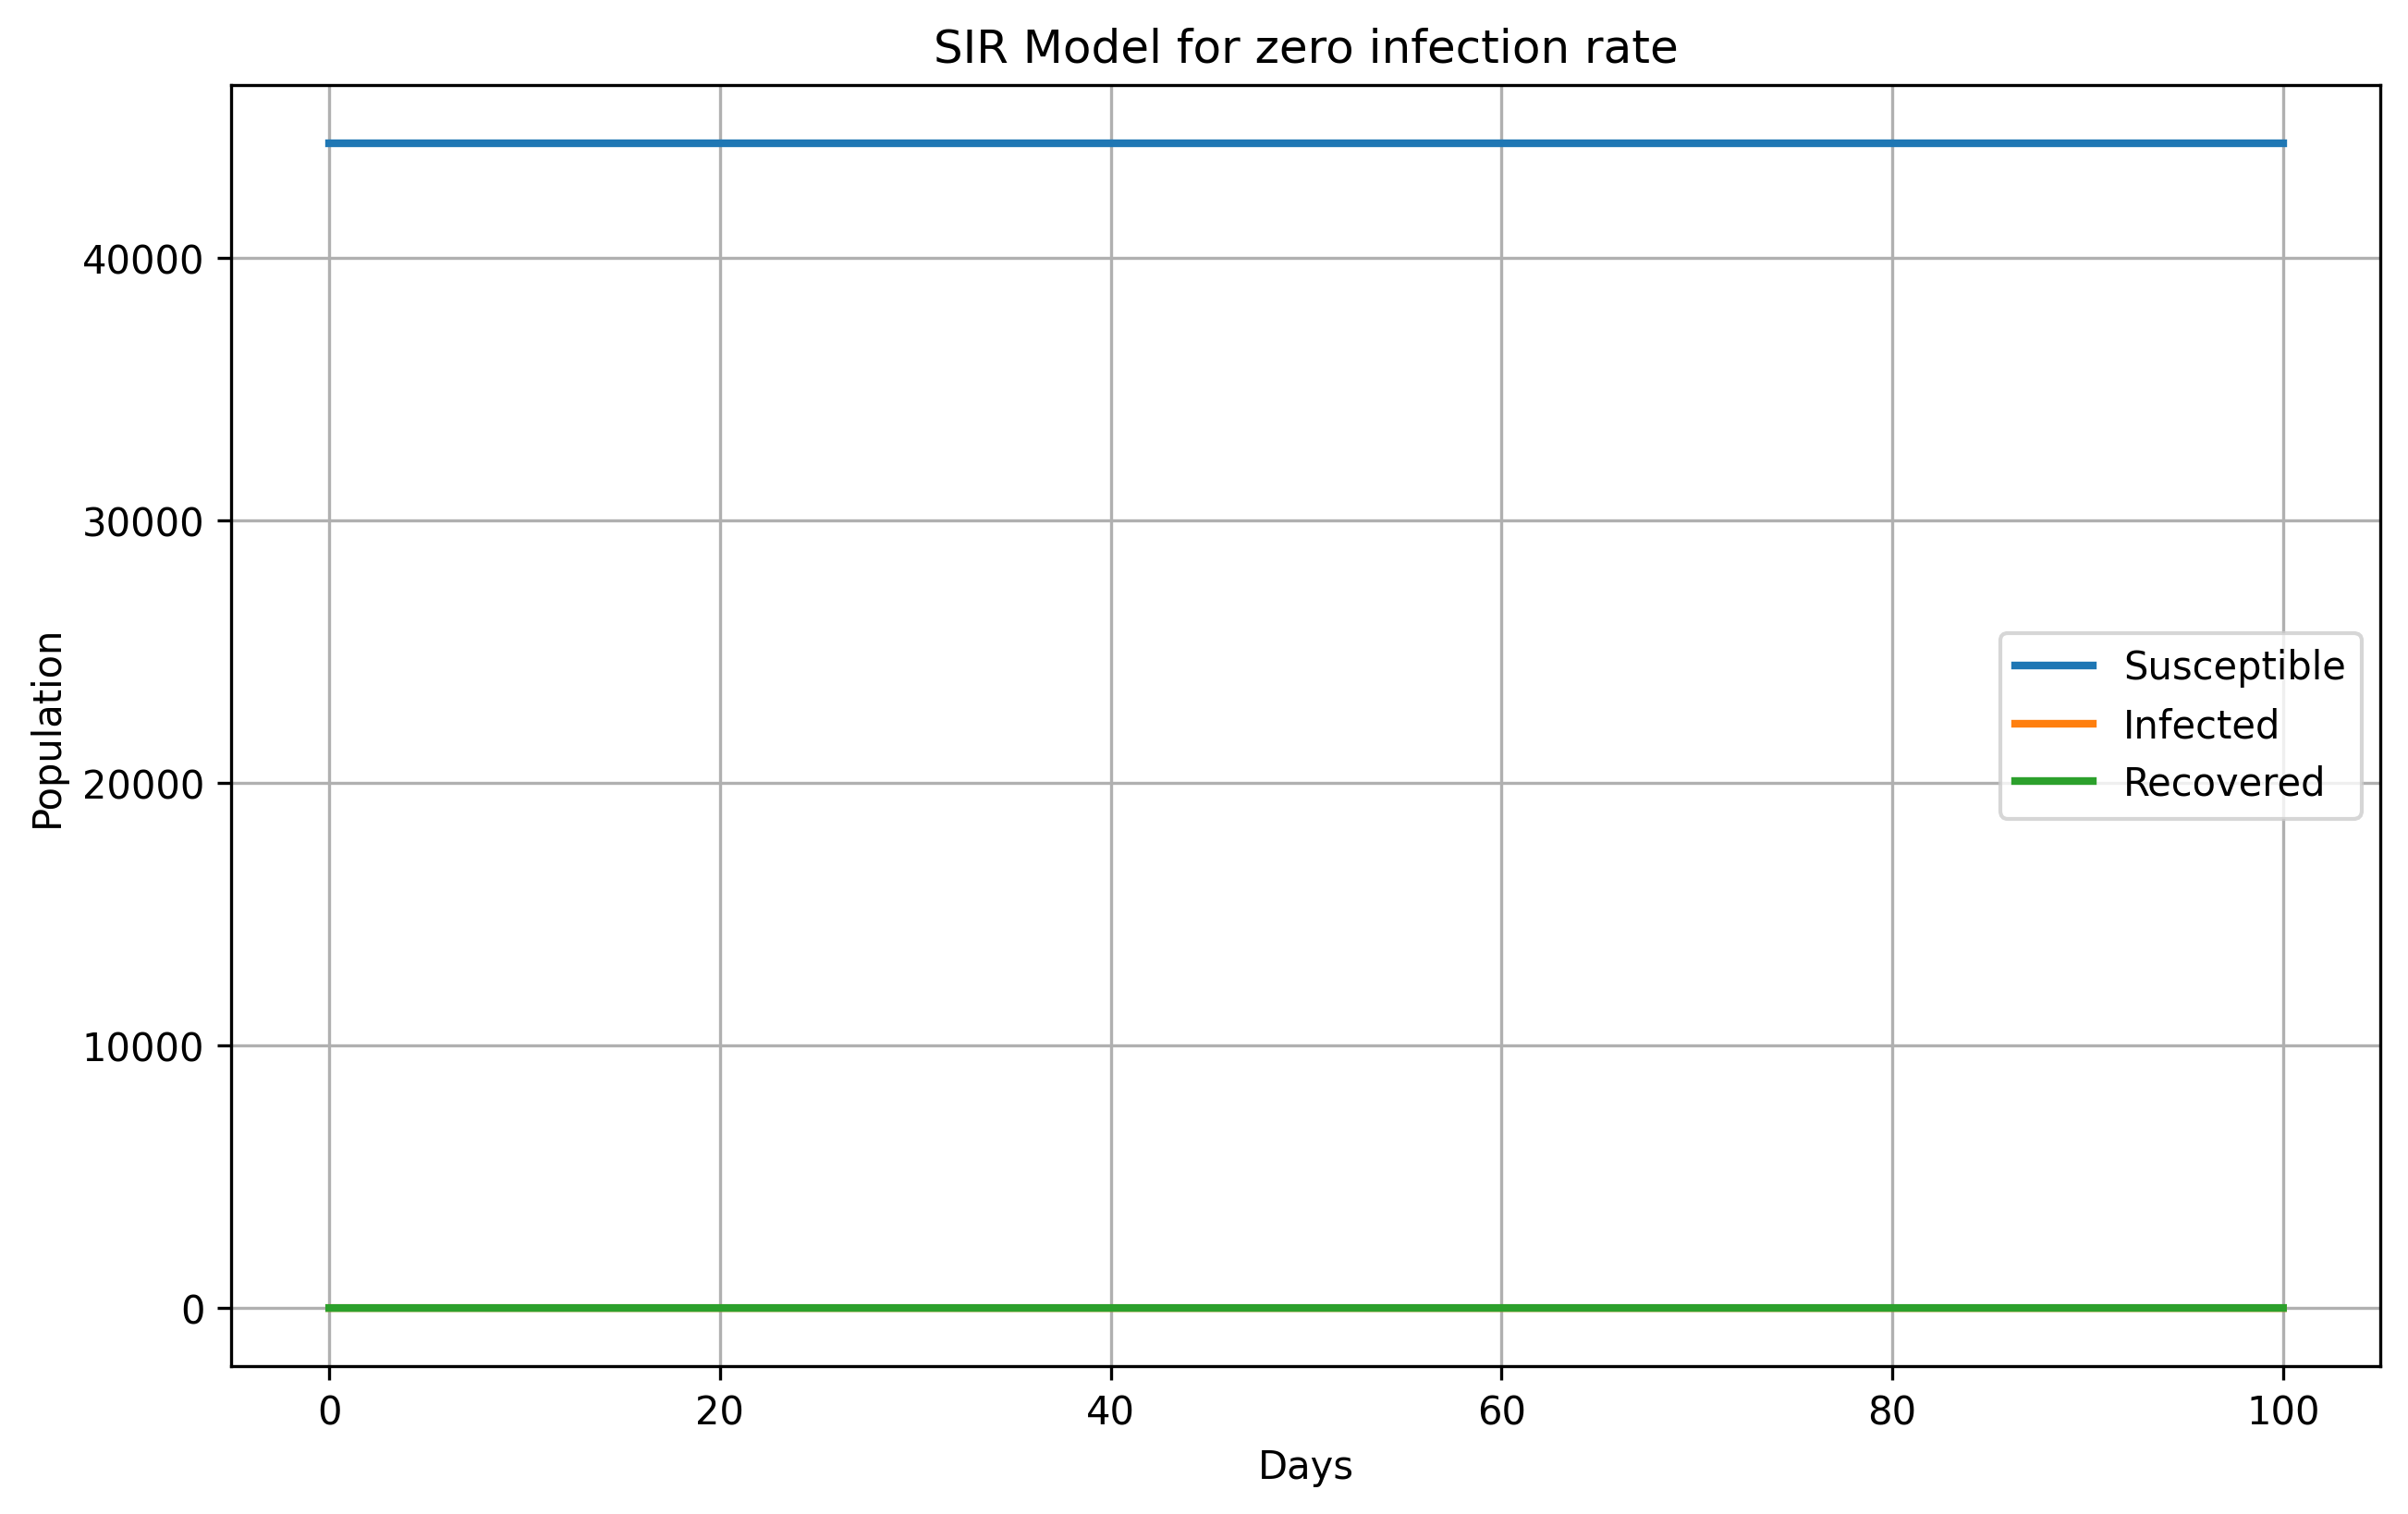
\includegraphics[width=0.5\textwidth]{zero_infection}
    \caption{Test case for zero infection rate}
    \label{zero_infection}
\end{figure}

\begin{figure}[H]
    \centering
    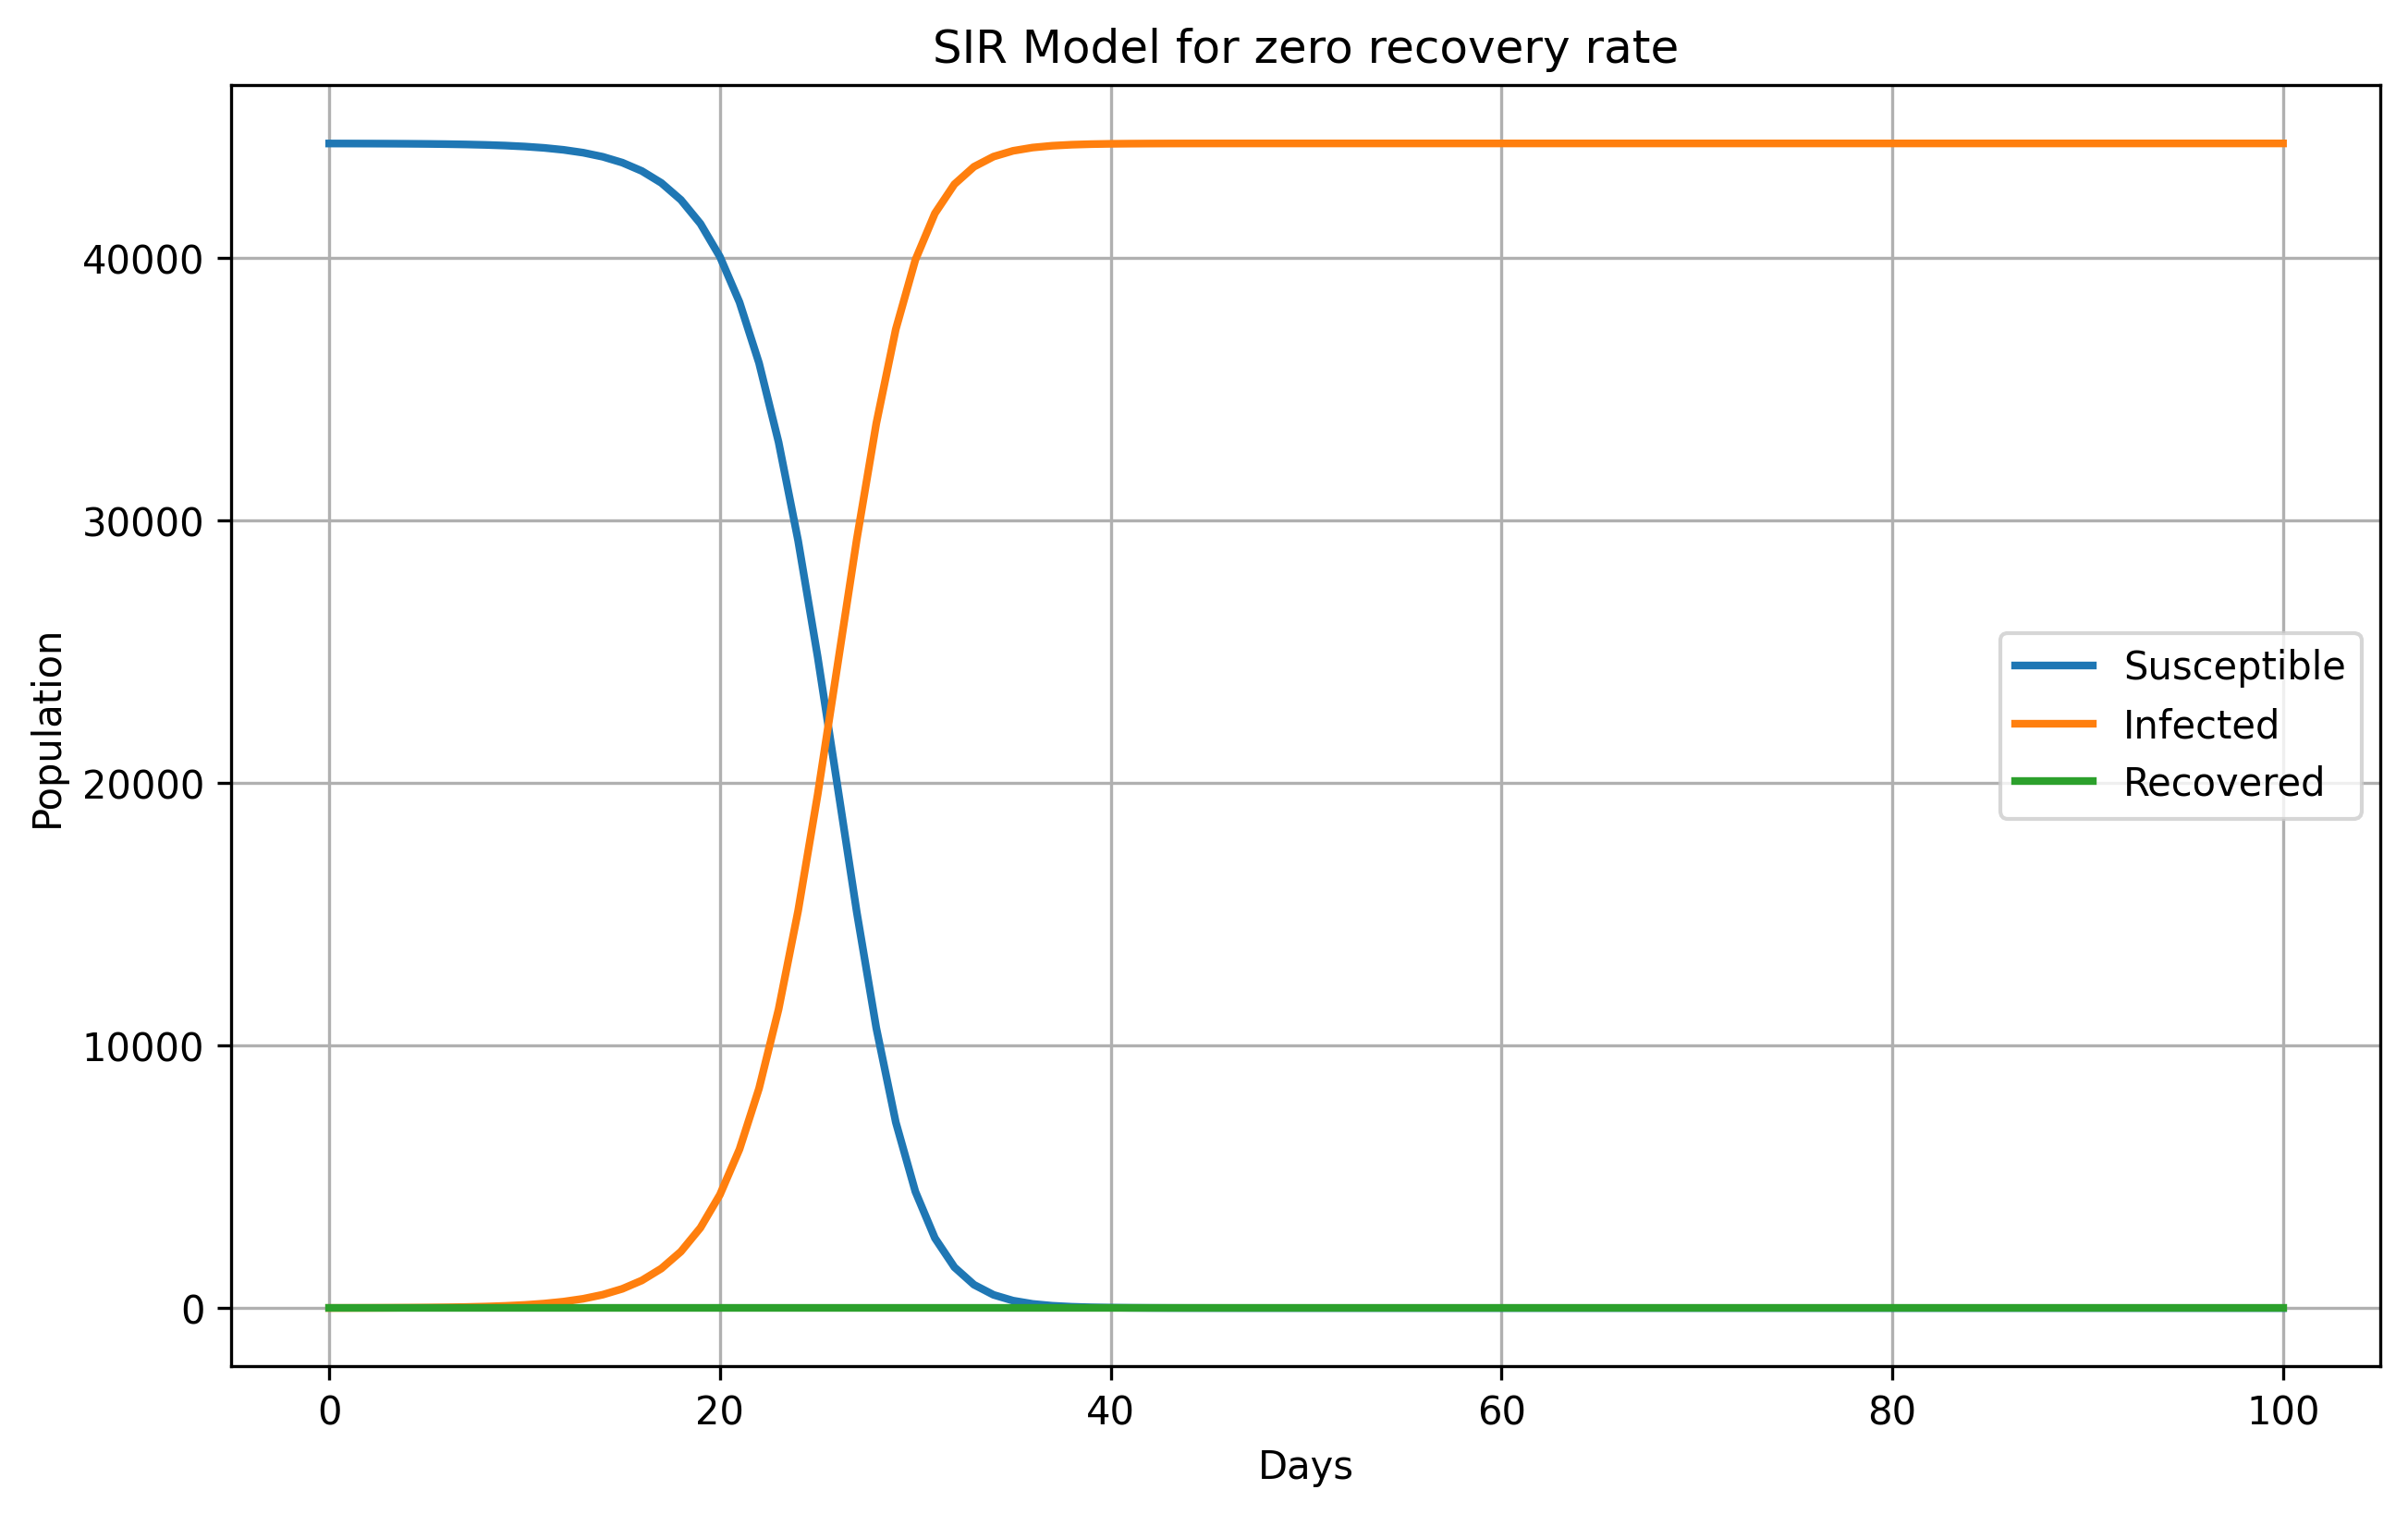
\includegraphics[width=0.5\textwidth]{zero_recovery}
    \caption{Test case for zero recovery rate}
    \label{zero_recovery}
\end{figure}

\subsection{Results}
Here is a simulation result for the following parameters:
$$
\begin{aligned}
    a & = 0.00001 \\
    b & = 0.025 \\
    S(0) & = 44358 \\
    I(0) & = 3 \\
    R(0) & = 0 \\
    t & = 100 \\
    time\_step & = 1
\end{aligned}
$$

\begin{figure}[H]
    \centering
    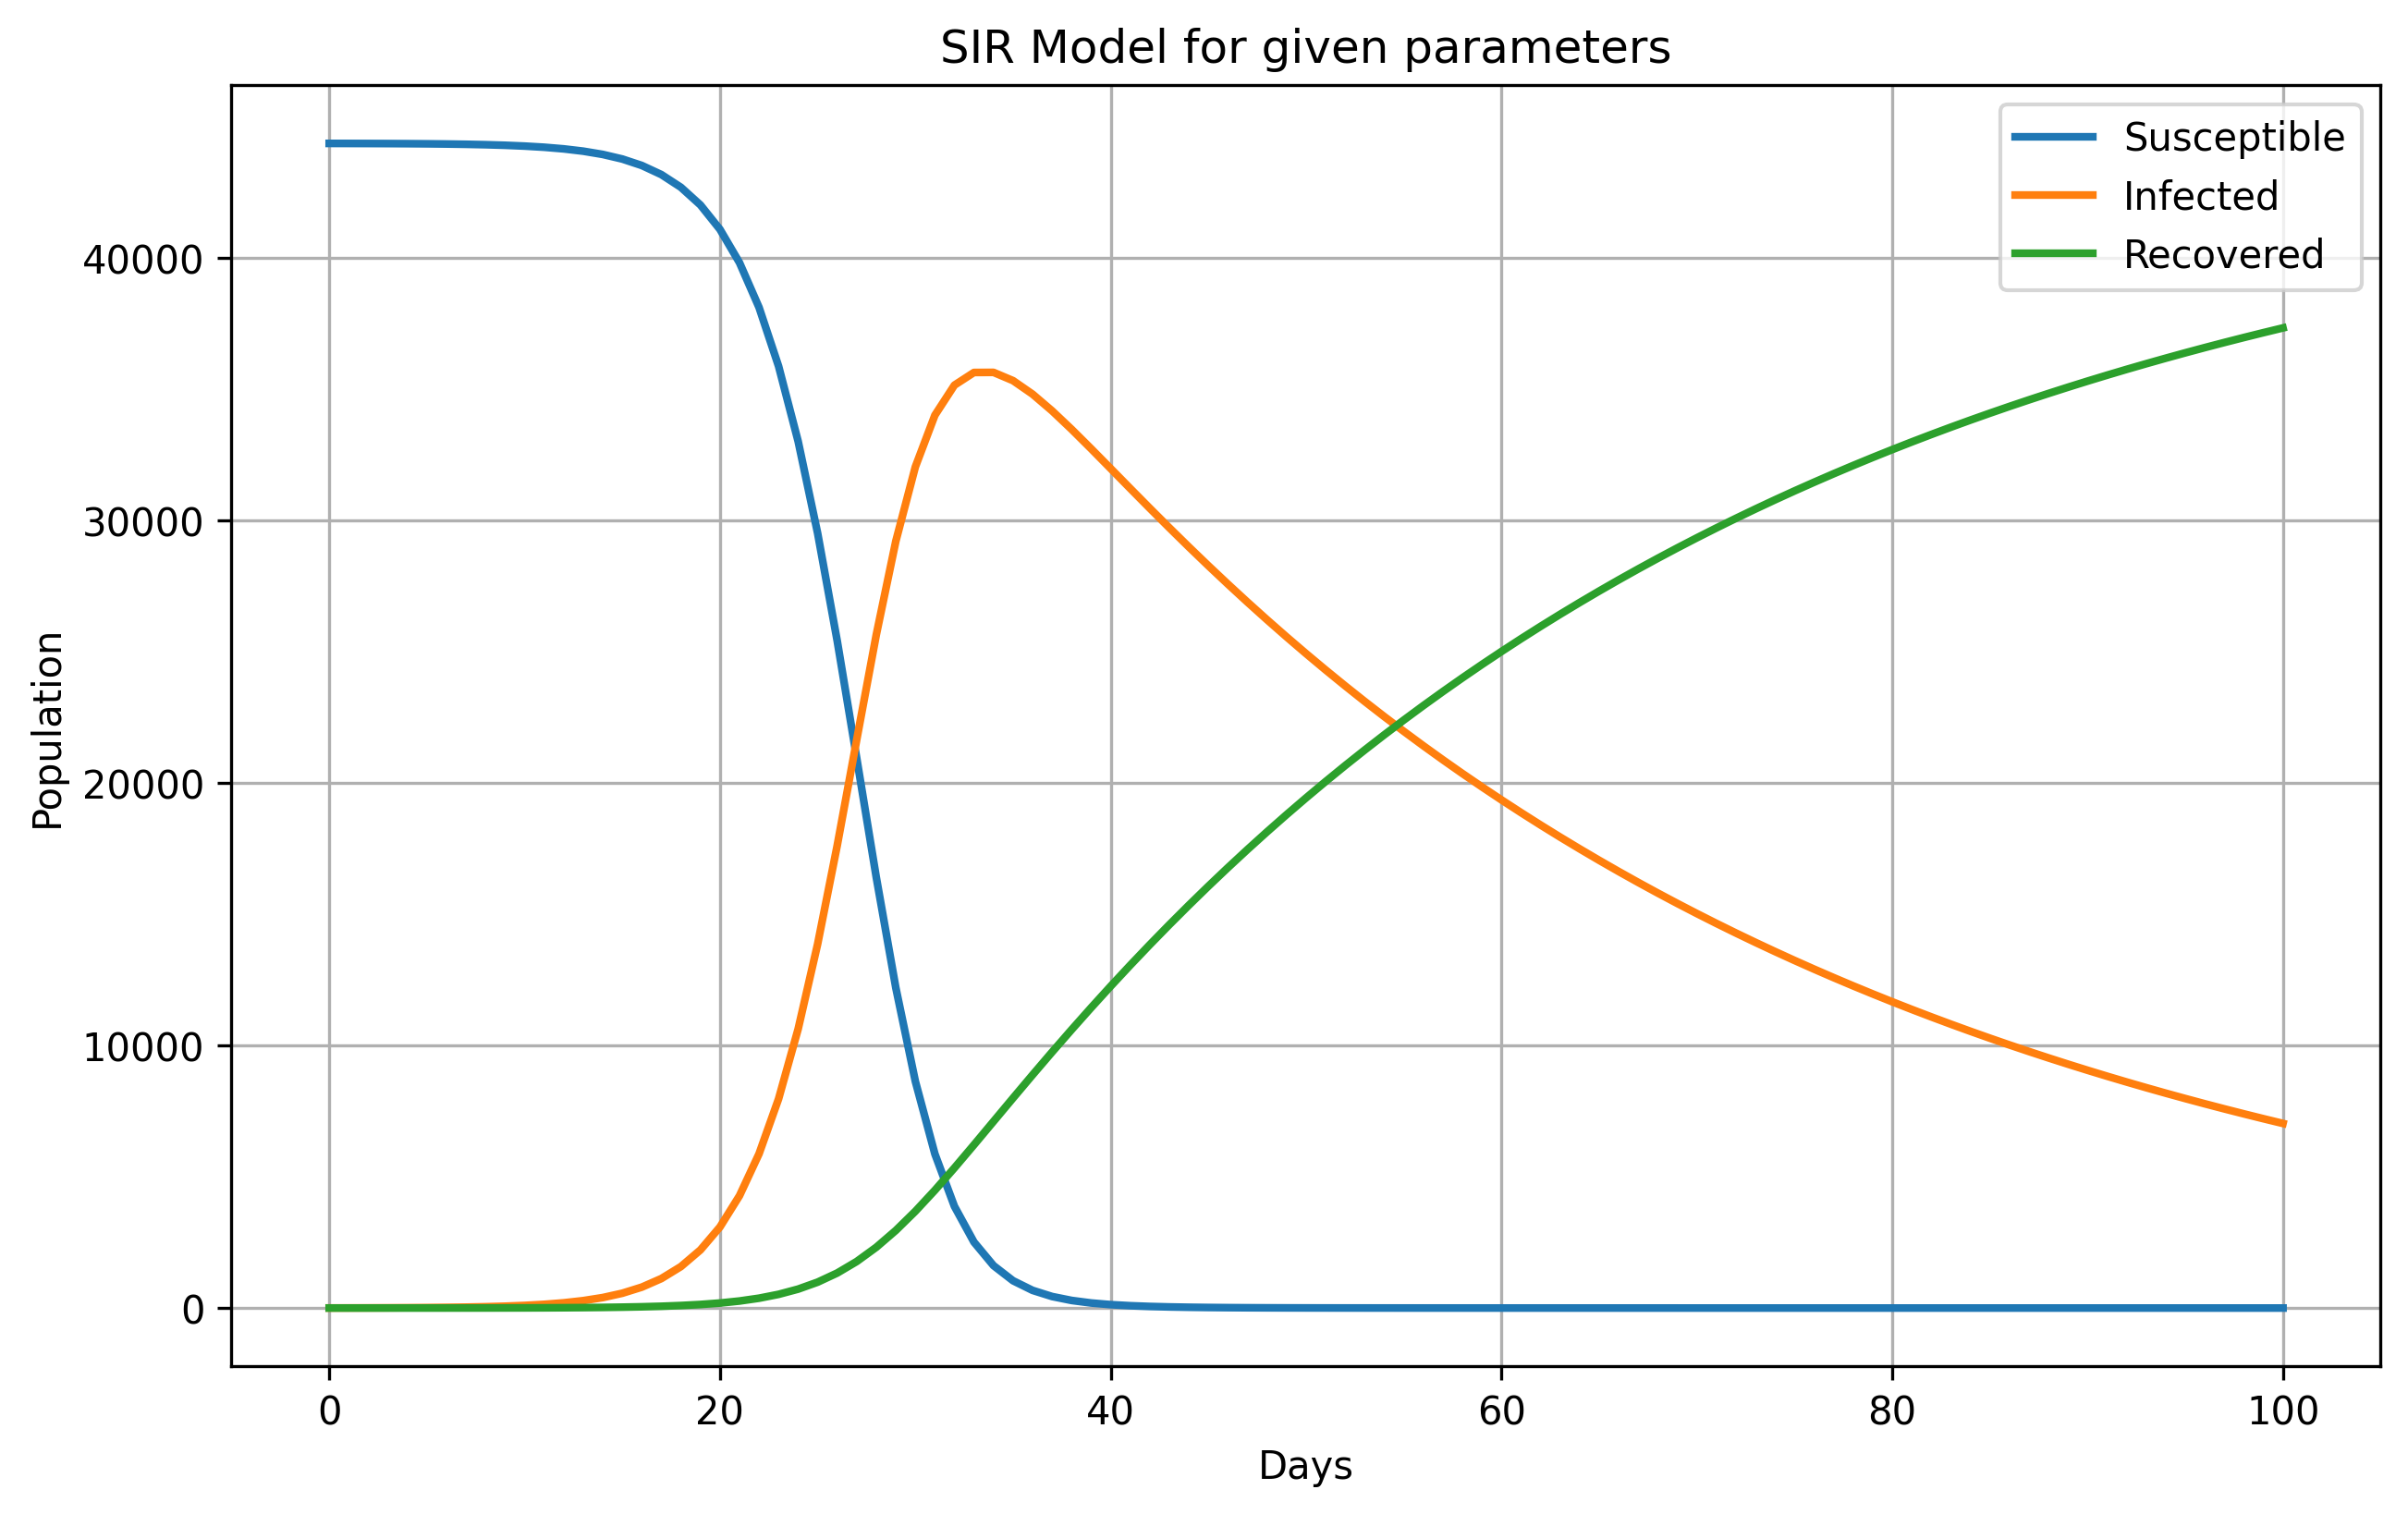
\includegraphics[width=0.5\textwidth]{given_parameters}
    \caption{Model result for given parameters}
    \label{given_parameters}
\end{figure}


\subsection{Probability Distributions}
To incorporate uncertainty in the parameters, I assumed the infection rate $a$ and recovery rate $b$ follow normal distributions: infection rate $a$ follows normal distribution with mean control value 0.00001 and standard deviation 20\% of the mean value; recovery rate $b$ follows normal distribution with mean control value 0.025 and standard deviation $\frac{1}{6}$ of the mean value. The following figures show the Infection number vs time with distributions in parameters.

\begin{figure}[H]
    \centering
    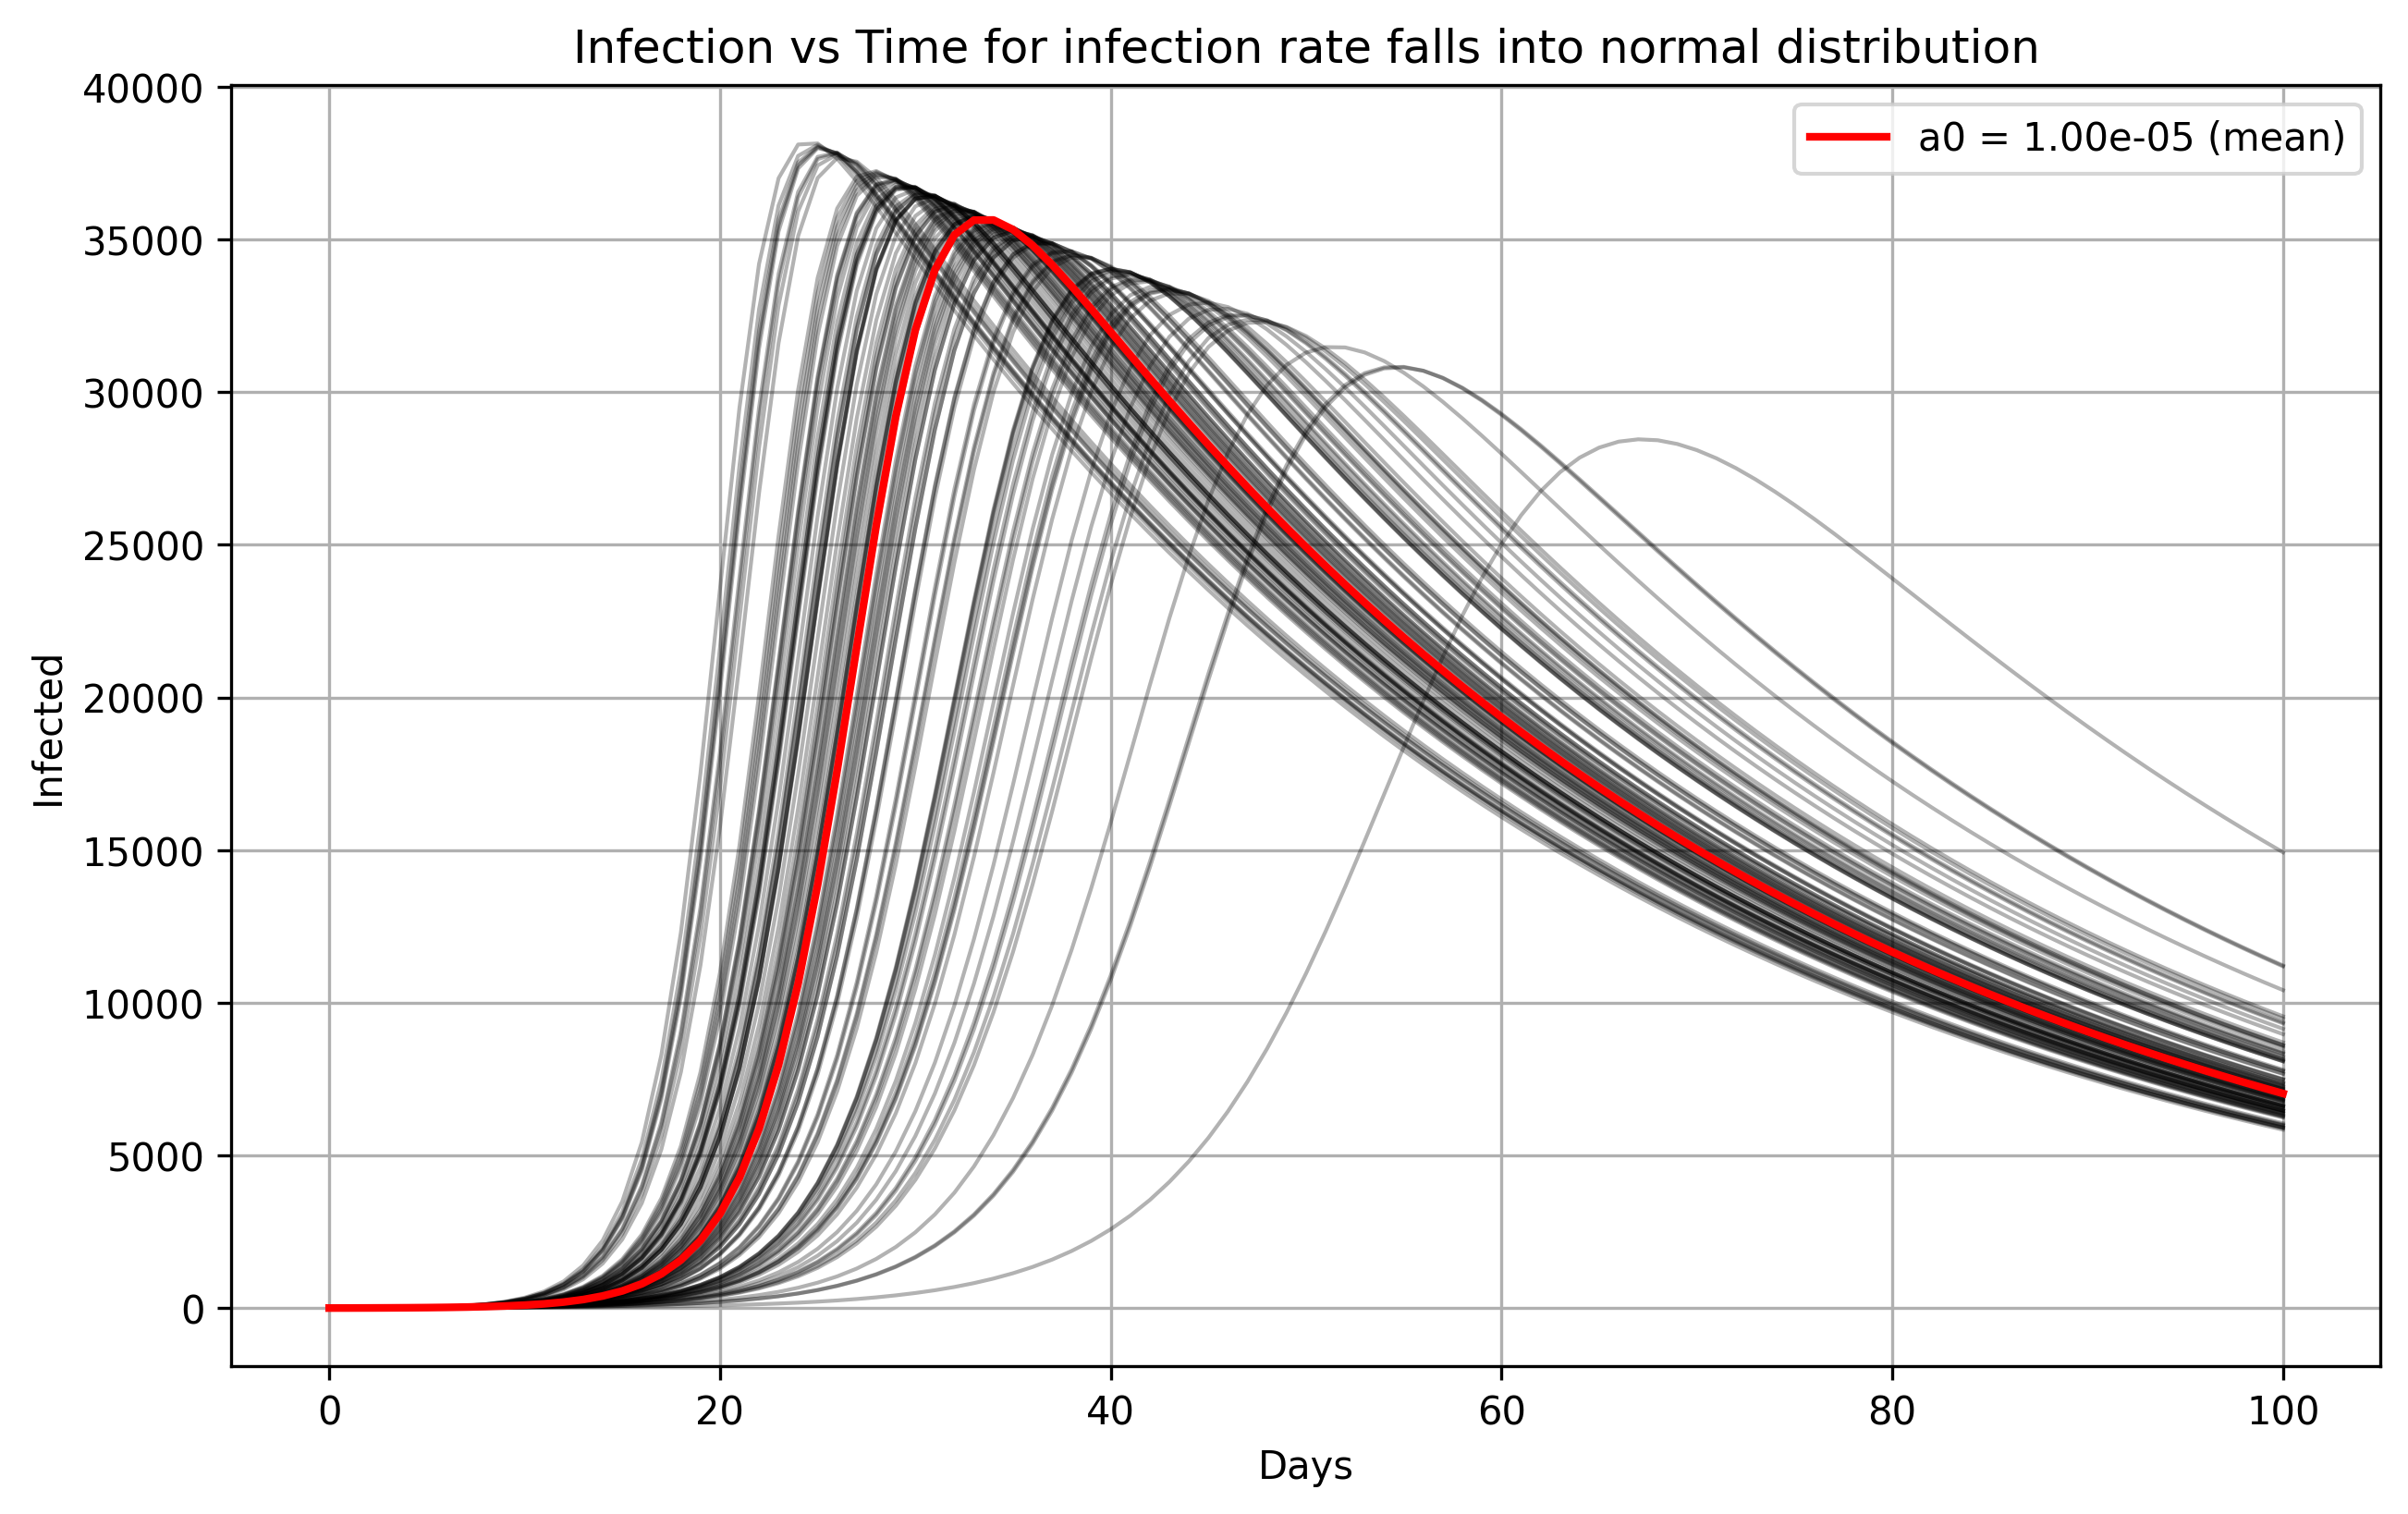
\includegraphics[width=0.5\textwidth]{infection_normal_distribution}
    \caption{Infection number vs time with distribution in infection rate $a$}
    \label{a_distribution}
\end{figure}

\begin{figure}[H]
    \centering
    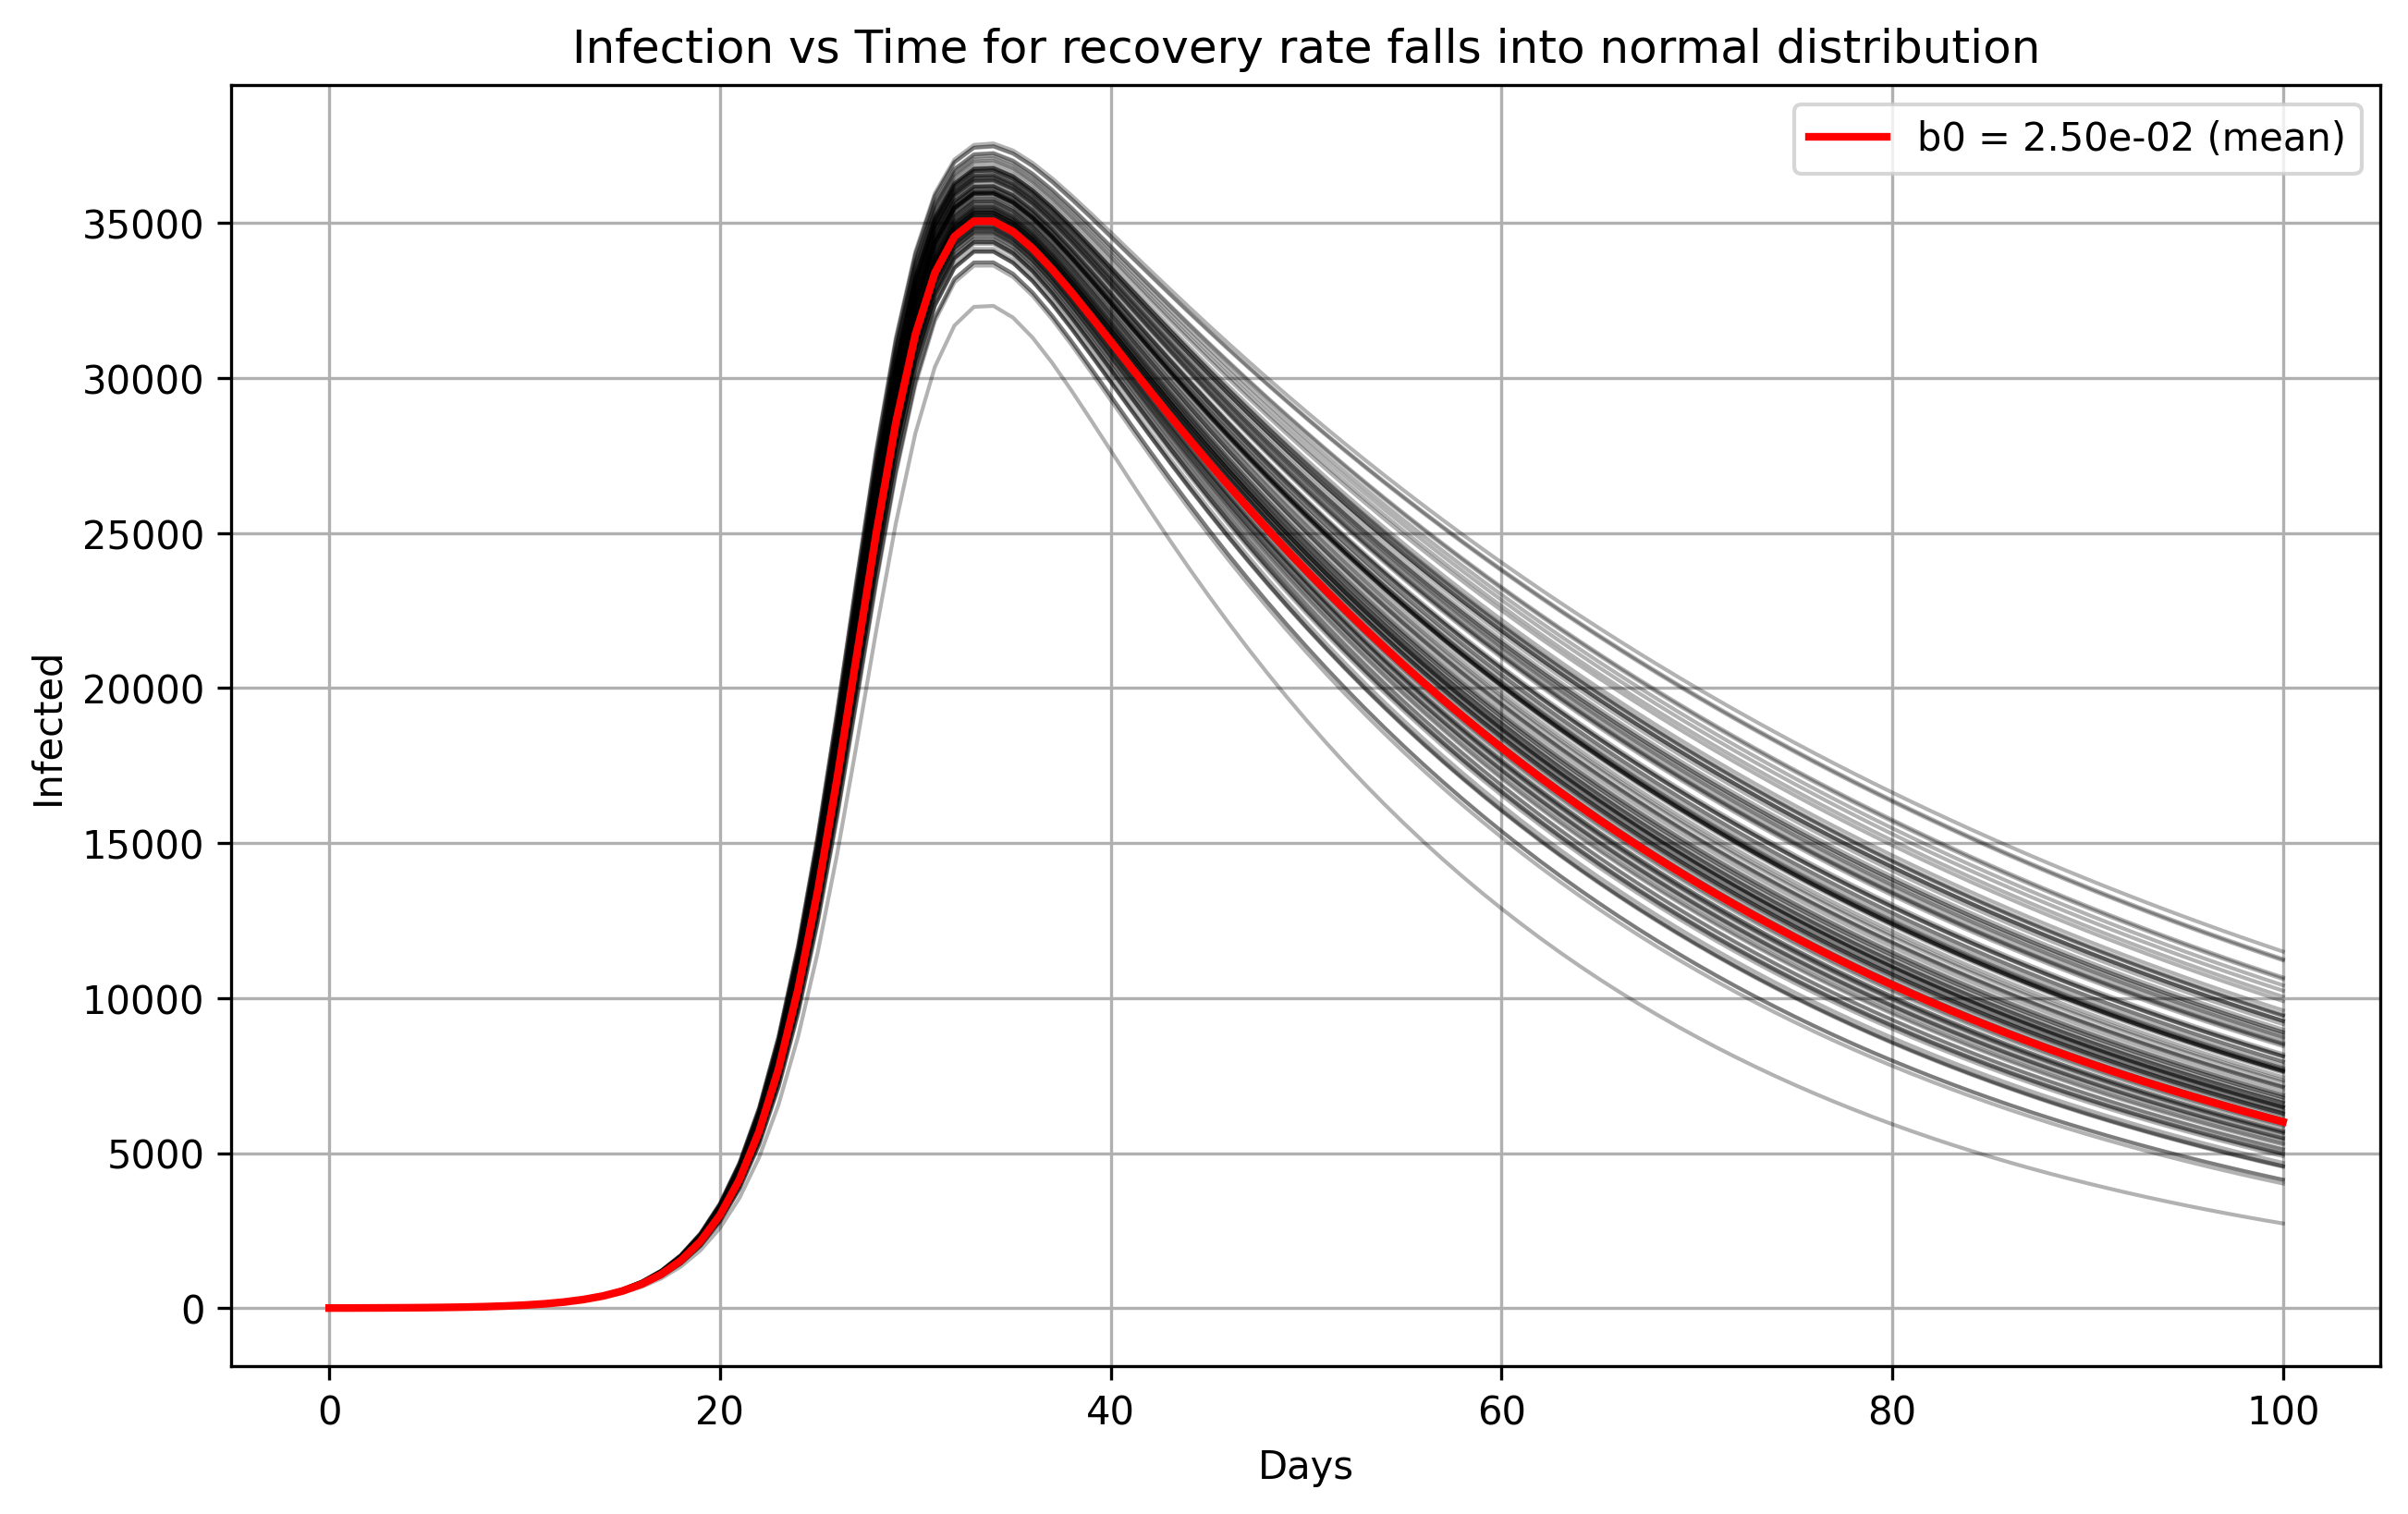
\includegraphics[width=0.5\textwidth]{recovery_normal_distribution}
    \caption{Infection number vs time with distribution in recovery rate $b$}
    \label{b_distribution}
\end{figure}

For both parameters following normal distributions at the same time, the following histogram shows the distribution of the maximum infection number during the simulation.
\begin{figure}[H]
    \centering
    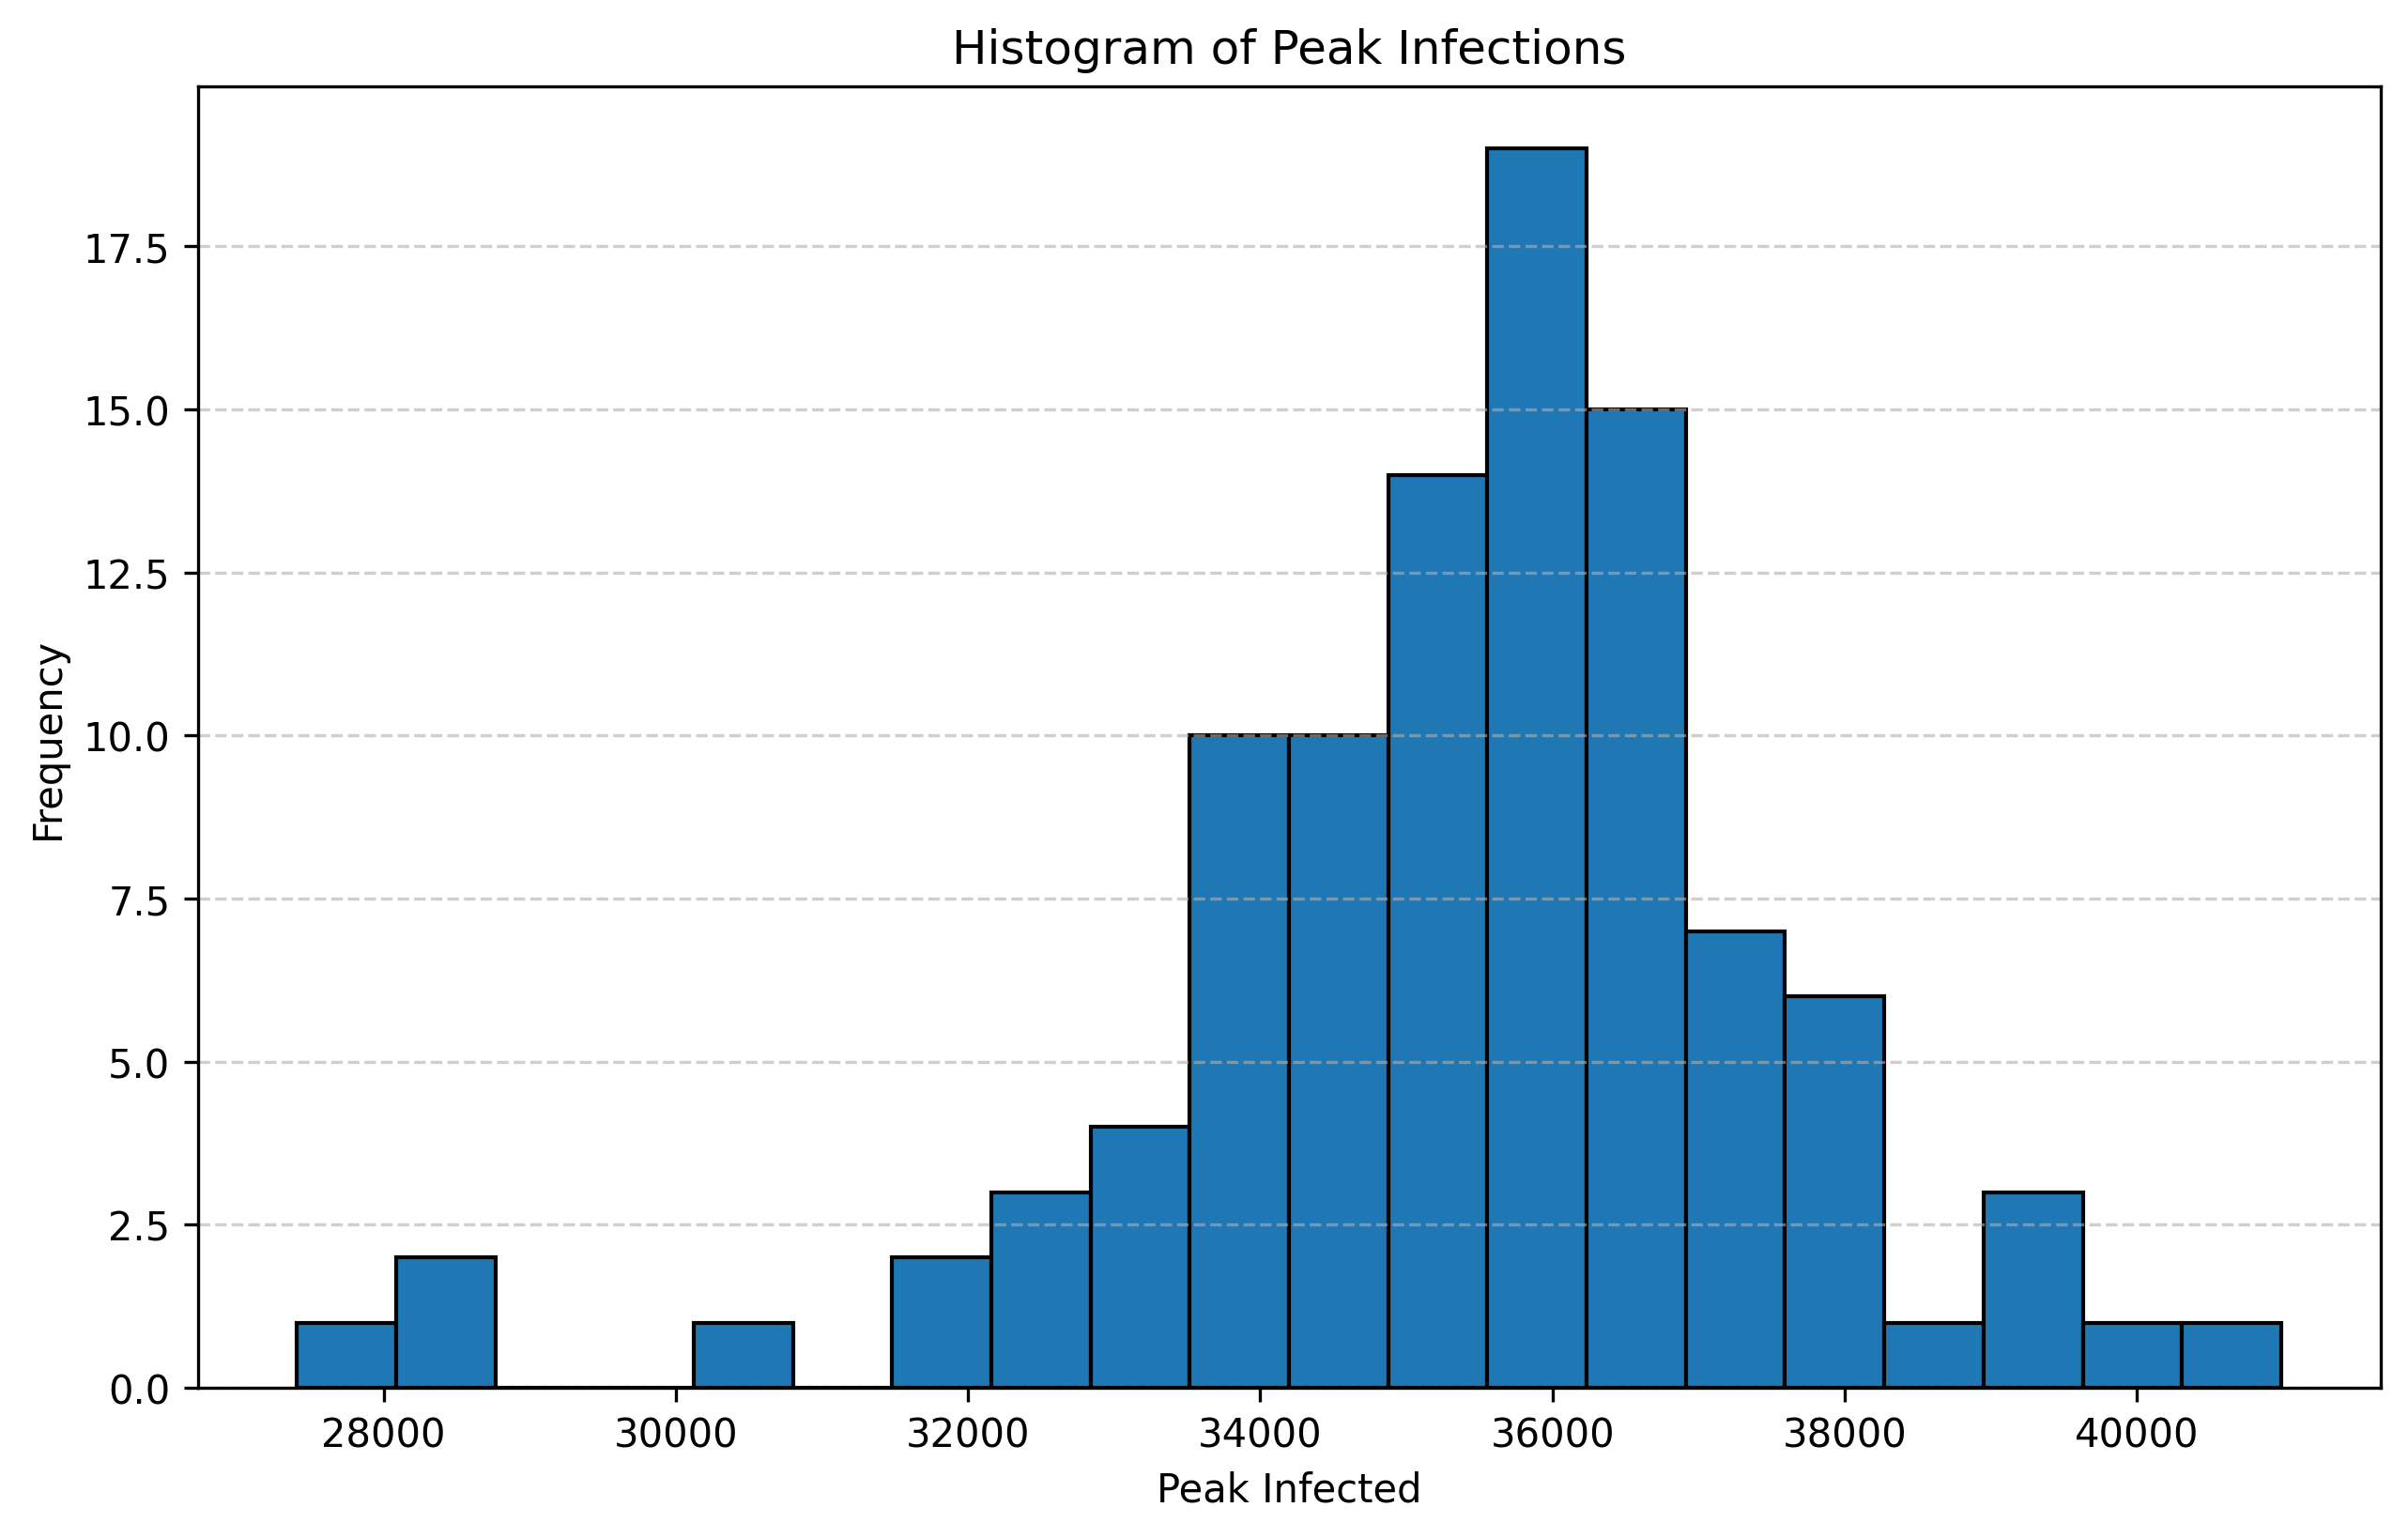
\includegraphics[width=0.5\textwidth]{histogram}
    \caption{Distribution of maximum infection number with both parameters following normal distributions}
    \label{histogram}
\end{figure}

\section{Conclusion}
This is a simple SIR model for the epidemic spreading based on the given data. The model can be further improved by incorporating more realistic assumptions and parameters.

\end{document}